\section{Pre-Configured Flexible Topology Design}
\label{sec:topology}

\begin{wrapfigure}{r}{230pt}
\centering
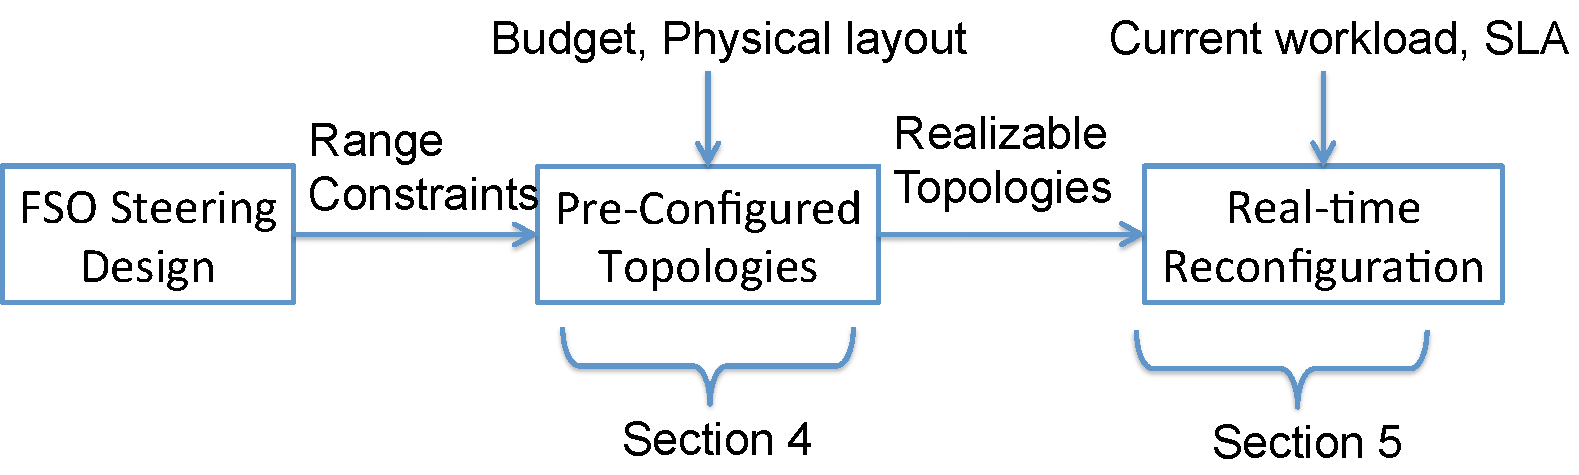
\includegraphics[width=220pt]{PPTFigs/OptimizationInteraction.pdf}
\caption{Interaction between the design constraints induced by FSO
steering choices, the selection of preconfigured topologies, and the
real-time topology selection} 
\label{fig:345}
\end{wrapfigure}

Design of the basic hardware elements of our architecture, discussed
in the previous section, impose certain physical constraints on our
overall architecture. For instance, the size of the FSO device
assembly limits the number of FSOs that can be placed on the rack. In
this section, we address the problem of designing an ``network
architecture'' with optimal performance, given the physical
constrants, pricing of hardware devices, and overall budget. See
Figure~\ref{fig:345}.
%
In essence, designing the network architecture entails determining the
network parameters (e.g., number of machines per rack, number of FSOs
per rack, number of FSOs with GM, number of SMs per FSO) and the
\blue{pre-orientation of GMs and pre-alignment of SMs}.  The
pre-orientation of GMs and pre-alignment of SMs in the system define
the set of {\em candidate links} (between pairs of FSOs). Note that,
during operation, only one candidate link is {\em active} per FSO at
any point of time. In essence, the set of candidate links defines a
set of {\em realizable network topologies}, of which {\em one} is
active/in-use at any point. The choice of active links (and hence, of
the {\em active topology}) in done is real-time based on the
prevailing traffic; this is handled by the {\em reconfiguration}
algorithm of our system, and is discussed in
Section~\ref{sec:reconfig}). See Figure~\ref{fig:345}.

We address the above problem of designing the network architecture
based on budget and physical constraints in following two
steps. First, to gain insights into the combinatorial and theoretical
nature of the problem, we address the \blue{concrete but also
  partly-abstract} problem of designing an optimal ``pre-configured
flexible topology'' given the number of racks, number of FSOs per
rack, and maximum number of candidate links per FSO (without reference
to GMs or SMs), and then in Section~\ref{sec:bbo} we use the
algorithm(s) for this problem to solve the budget-based network
architecture design optimization problem.

\subsection{PCFT Problem}

Given the number of racks $n$, number of FSOs $m$ on each rack, and
the maximum number of {\em candidate links} $k$ per FSO, the {\bf {\em
    pre-configurated flexible topology (PCFT) design problem}} is to
determine the set of candidate links for each FSO, so as to optimize
the ``dynamic bisection bandwidth'' of the network (as defined below).

\softpara{Rethinking Metrics: Dynamic Bisection Bandwidth (DBW).}  The
traditional bisection bandwidth metric reflects a {\em static}
perspective of the topology. However, in our context, we should
instead consider the notion of {\em dynamic} bisection bandwidth (DBW)
since different realizable topologies can be used for different
communication requirements. Formally, the dynamic bisection bandwidth
of a given pre-configured topology $\Pi$ can be defined as
follows. Let $T$ be the set of realizable topologies of a given
pre-configured topology $\Pi$, $P$ be the set of partitions of the
given network into \blue{two equi-sized sets of machines}, and
$BW(t,p)$ be the bandwidth of the topology $t$ for the partition $p$.
Then, the {\em dynamic bisection bandwidth} for the pre-configured
topology $\Pi$, denoted by DBW($\Pi$), is defined as:

$${\rm DBW}(\Pi)  = \min_{p \in P} (\max_{t \in T} {\rm BW}(T, p)).$$

In addition to bisection bandwidth, a bound on worst-case latency
between pairs of network nodes has also been considered as an
objective in designing datacenter topologies~\cite{rewire-20-39}.
Worst-case latency can be approximated by the network diameter. In our
context, we can define an appropriate notion of {\em dynamic diameter}
(as for DBW above), and consider maximizing DBW under the constraint
of bounded (dynamic) diameter.

Finally, if we have some coarse statistics available on the expected
inter-rack traffic, then we can use it to tailor our DBW objective
accordingly. Note that since pre-configuration can only be done on an
infrequent basis (e.g., weekly), so we are only interested in coarse
traffic knowledge; the near-term traffic information is instead used
for reconfiguring the network (discussed in
Section~\ref{sec:reconfig}). One simple form of inter-rack traffic
statisfics could be in the form of a weights between every pair the
racks, and the DBW definition can be appropriately tailored as
in~\cite{leighton-99} for multi-commodity min-cut. \blue{In our
  research, we will also consider more sophisticated stochastic
  traffic models~\cite{}.}

\softpara{Connection to Known Graph Problems.}  In general, the PCFT
problem is in the class of the {\em network design problem
  (NDP)}~\cite{ndp-survey}, wherein the goal is to extract a subgraph
satisfying some design criteria and optimizing a given objective
function. More specifically, the PCFT problems falls in the class of
{\em degree-constrained subgraph} problems~\cite{degree-survey}
wherein the extracted subgraph is constrained by the degree on each
vertex. What distinguishes the PCFT problem from the prior-addressed
NDP problems is the choice of our objective function, viz., dynamic
bisection bandwidth.

Note that the PCFT problem under DBW maximization is very different
from the well-known NP-hard problem of {\em computing} the bisection
bandwidth of a {\em given} graph~\cite{}. The special case of the PCFT
problem, when $k=1$, actually boils down to constructing an
$m$-regular graph over $n$ nodes with maximum (static) bisection
bandwidth. The closely known problems to this $k$=1 case of our
PCFT problem are:

\squishlist
\item
{\em Finding} the bisection bandwidth of a given regular graph; this
problem is known to be NP-hard~\cite{bui-leighton-comb-1987}, with the
best known approximation-factor of $O((\log n)^2)$~\cite{fiege-focs-2000}.

\item
Determining an {\em upper-bound} on the bisection bandwidth of
$m$-regular graphs of size $n$, for a given $m$ and $n$. Note that
this problem can be reduced to the $k=1$ version of our PCFT
problem. This upper-bound problem has been addressed extensively, and
upper-bounds have been determined for small values (upto 4) of
$m$~\cite{monien-2006}; these upper-bound results are not tight.
\squishend

The above results suggest that, even for $k=1$, the PCFT problem is
likely to be intractable. In general, the PCFT problem can be thought
of as the following graph problem: Given $n$, $m$, and $k$ (as defined
in the formulation), the PCFT problem is to find a $k$-regular graph
over $nm$-nodes such that the {\em set} of matchings (i.e., realizable
topologies) in the graph maximizes the dynamic bisection andwidth. To
the best of our knowledge, the above graph problem (or anything
closely related) has not been addressed before.

\begin{task}
\label{task:pcft}
We will design efficient algorithms for the Pre-Configured Topology
Design problem with the objective of maximizing dynamic bisection
bandwidth.
\end{task}

\para{Proposed Approaches.} We will pursue the following approaches
for the PCFT problem:

\softpara{Static to Dynamic Conversion.} One reasonable approach to
solve the PCFT problem would be to start with constructing a
$km$-regular graph of $n$ nodes with a high (static) bisection
bandwidth, and then group the $km$ candidate links at each node into
$m$ sets of $k$ links each so as to maximize the dynamic bisection
bandwidth. For the \underline{first step}, there are only a few
results on explicit construction of general graph classes with high
bisection bandwidth~\cite{peres}. In particular, $d$-regular Ramanujan
Graphs~\cite{rewire-18} of are known to have a bisection width of at
least $((d/2 - \sqrt(d-1))n/2$, but their construction is mostly
algebraic. Other graph classes of interest are Cage graphs, which are
minimum girth~\cite{cage}. In our specific context of small values (a
few hundreds) of $km$ and $n$, we can investigate bisection bandwidth
of certain classes of regular graphs, and pick ones that suggest a
high bisection bandwidth \blue{with low diameter}; in particular, due
to symmetry of nodes/racks, we can also restrict ourselves to
``symmetric'' regular graph such as distance-transitive graphs. For
the \underline{second step} of grouping candidate links, we will
employ certain heuristics. E.g., we can number the $n$ nodes from 1 to
$n$ and group the $km$ links into the $m$ sets based on the ranges of
node numbers they connect to. Such a heuristic will guarantee a
``uniform'' division of links into sets across the nodes.

\softpara{Dual-based Approach.}  If each rack contains $l$ machines
and the links (between a machine and the ToR switch, or a pair of
FSOs) have a unit bandwidth, then the optimal desired bisection
bandwidth is $nl/2$. \blue{We note that inter-rack and inter-machine
  bisection bandwidths are the same for uniform link bandwidths.}
%
Now, let us consider what values of $k$ and $m$ can enable this DBW
value of $nl/2$. We consider two extremes: (a) If $k=1$, then it can
be shown that \blue{$m = \min(n/2+l, 7l)$ suffices (but not
  necessarily optimal).} For large values of $n$ and $l$, it is
known~\cite{book-28-29} that $m=2l$ would almost always work. (b) If
$k$ can be an arbitrarily high, then the optimal value of $m$ required
is $l$ (for $k=n/2$); here, for $m=l$, the $k$ required (=$n/2$) is
also optimal. The above resuls hold for any DBW value that is an
integral multiple of $n$.
%
The above near-optimal solutions for certain special cases of the
``dual'' problems (i.e., given a desired DBW value, minimize $m$ or
$k$ for a given $n$ value) gives us some insights into solving the
PCFT and its dual problems.  In particular, if we can solve the above
dual problem of minimizing $m$, given $k$, $n$, and a desired DBW
value, for arbitrary $k$ values and integral of $n$ values of DBW,
then it is easy to derive an approximation algorithm for the PCFT
problem that has only an {\em additive} approximation-factor of $n$.

\softpara{Simulated Annealing.}  Simulated Annealing (SA)
heuristics~\cite{} have been used with great success for optimization
problems. To design a simulated annealing approach for our PCFT
problem, we need three key components: {\bf (a)} A good ``seed''
(starting) solution; here, we could use one of our earlier approaches,
or as in~\cite{rewire}, use graphs with a ``large spectral
gap''~\cite{rewire,spectral,rewire-18} which are known to have
desirable properties (e.g., low diameter~\cite{spectral-diameter}).
{\bf (b)} Ways to generate ``neighboring'' solutions; for this, we can
use \blue{simple transformations} that transform a regular graph to
another. E.g., the transformation that changes the edges ${(a,b),
  (c,d)}$ to ${(a,c), (b,d)}$ can be used iteratively to construct any
regular graph from another.  {\bf (c)} An efficient heuristic for
computing DBW of a given graph; for this, we will investigate
generalization of the following approaches: (i) Well-known efficient
heuristics, viz., SA~\cite{} and Kernighan-Lin~\cite{} for computing
the bisection bandwidth, and (ii) a recent result~\cite{rewire} that
uses Valiant (or, two-state) load balancing technique~\cite{valiant}
to compute a {\em lower bound} on the bisection bandwidth. \blue{The
  above ideas can also be appropriately extended to optimize the
  traffic-weighted DBW objective.}


\subsection{Budget-Based Optimization}

\begin{task}
\label{task:bbo}
We will design efficient algorithms for the Budget-Based Optimization
Problem with the objective of maximizing dynamic bisection bandwidth.
\end{task}

We now consider the budget-based optimization (BBO) problem mentioned
at the start of the section. Formally, given the number of machines
($N$) to interconnect, physical constraints, overall budget, and
pricing of relevant hardware devices, the BBO problem is to determine
the following such that the dynamic bisection bandwith is maximized:
(a) Number of machines ($l$) per rack and thus, the number of racks
($n = N/l$), (b) number of FSOs ($m$) per rack and thus, the number of
ports (=$m+l$) on the ToR switch, (b) Number of FSOs ($m_1 \leq m$)
that are each equipped with a GM and the number of SMs (k') on each of
the remaining $(m-m_1)$ FSOs, on each rack, and (c) the {\em
  pre-orientation} of each of the GMs and {\em pre-alignment} of each
of the SMs in the system.

Based on our insights from the previous section, we will use the
following approaches to address the BBO problem:

\squishlist
\item
{\em Using PCFT Algorithm.}  To use PCFT problem: {\bf (a)} First, we
convert the given budget and physical constraints, and the pricing
information into a constraint equation over $n$ (number of racks), $m$
(number of FSOs per rack), and $k$ (the number of candidate links per
FSO). To relate $k$ to the parameter $k'$ of the problem, we need an
an additional variable $f$ (the fraction of FSOs on each rack equipped
with a GM) and a constant $c$ (number of candidate links a GM can be
steered to use). I.e., we use $k = fc + (1-f)k'$.
%
{\bf (b)} Second, we solve the PCFT problem for various $n$, $m$ and $k$
that satisfy the above budget constraint for a given $f$. Convert each
PCFT solution to a design realizable by $fm$ GMs and $(1-f)m$ sets of
$k$ SMs each, on each rack, and estimate its DBW using one of the
approaches described earlier. {\bf (c)} Lastly, we explore the space of
$n,m,k,f$ efficiently using standard search techniques, to compute an
efficient network design for the given budget and pricing.

\item
{\em Simulated Annealing Approach.}  We can modify our Simulated
Annealing approach described above for the PCFT problem to solving the
BBO problem, by appropriately modifying the transformation operator to
generate neighbors of a particular network design. Here, the neighbors
of a design may include designs with slightly different values of
parameters $n$, $m$, $k$, $f$, and/or candidate links, under the
budget constraints.  
\squishend
